\section{Auswertung}
\label{sec:Auswertung}
Jegliche Fehlerrechnung wurde mit der python-Bibliothek uncertainties \cite{uncertainties} absolviert.
Allgemeine Rechnungen wurden mit der python-Bibliothek numpy \cite{numpy} automatisiert. 
Die graphischen Unterstützungen wurden mit Hilfe der python-Bibliothek matplotlib \cite{matplotlib} erstellt.\\
\subsection{Berechnung der Energien der charakteristischen Linien} \label{sec:energy}
In der Abbildung \ref{fig:copper} sind die gemessenen Impulse N gegen den Winkel $\theta$ aufgetragen.
Aus dieser Graphik geht hervor, dass die $K_\beta$ Linie bei einem Winkel von $\theta_\beta = \ang{20.2;;}$ mit 
N$=1599$ Impulsen liegt.
Die $K_\alpha$ Linie liegt bei einem Winkel von $\theta_\alpha = \ang{22.5;;}$, wo
N$=5050$ Impulse gemessenen wurden.
Für die Energien wird die Gleichung \eqref{eqn:bragg} benötigt.
Um auf die Energien schließen zu können wird die Beziehung $E = \sfrac{hc}{\lambda}$ benötigt.
Somit kann mittels 
\begin{equation}
    E = \frac{hc}{2 d \sin \theta}
\end{equation}
die Energie berechnet werden.
Mit der Beugungsordnung $n = 1$, der Lichtgeschwindigkeit $c = \SI{299792458}{\metre\per\second}$\cite{speedoflight},
dem Plank'schen Wirkungsquantum $h = \SI{6.626e-34}{\joule\second}$\cite{plank}
und einer Gitterkonstante des LiF-Kristalls von $d=\SI{201.4}{\pico\metre}$ ergeben sich die Energien der Linien zu
\begin{align*}
    E_\beta &=\SI{8.92}{\kilo\electronvolt} \\
    E_\alpha&=\SI{8.04}{\kilo\electronvolt} 
\end{align*}
\begin{figure}
    \centering
    \caption{Emissionsspektrum der Kupfer Röntgenröhre.}
    \label{fig:copper}
    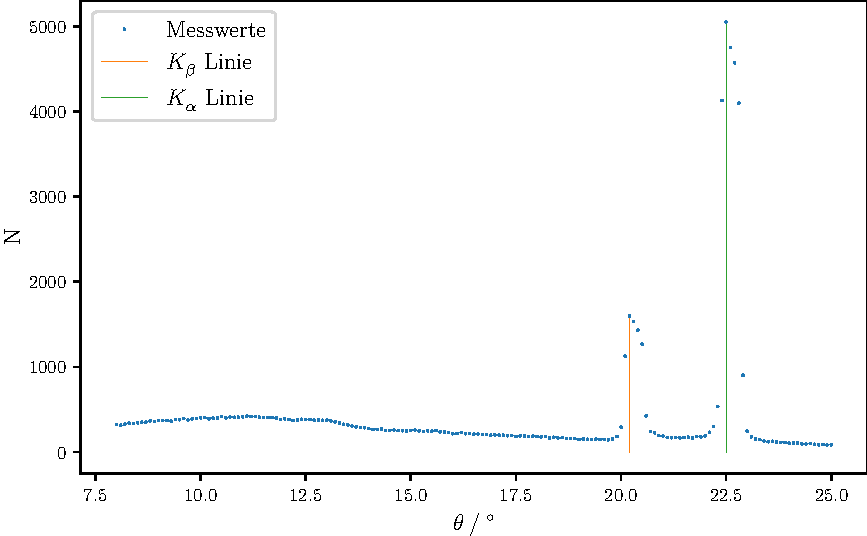
\includegraphics{build/copper.pdf}
\end{figure}
\FloatBarrier
\subsection{Bestimmung der Transmission} \label{sec:transmission}
In der Tabelle \ref{tab:mess} sind die gemessenen Zählraten ohne Aluminium-Absorber $N_\text{o}$ und mit Aluminium-Absorber $N_\text{Al}$ 
mit den daraus berechneten Transmissionen $T$
in Abhängigkeit von dem Winkel $\theta$ aufgetragen.
Bevor die Transmission mit $T = \sfrac{I_\text{Al}}{I_\text{O}}$ berechnet werden kann,
müssen die Zählraten mit Hilfe der Totzeitkorrektur\eqref{eqn:tot} korrigiert werden.
\begin{table}
    \centering
    \caption{Gemessene Impulsraten mit den dazugehörigen Transmissionen.}
    \label{tab:mess}
    \begin{tabular} {S[table-format=2.1] S[table-format=3.1] S[table-format=3.1]  
      S[table-format=1.3] @{${}\pm{}$} S[table-format=1.3]}
    \toprule
    {$\theta \mathbin{/} \si{\degree}$} & {$N_\text{o}$} & {$N_\text{Al}$} &
    \multicolumn{2}{c}{$T$}\\
    \midrule
    7.0	& 226.0 & 113.5 & 0.497 & 0.005 \\
    7.1	& 232.0 & 112.0 & 0.477 & 0.005 \\
    7.2	& 240.5 & 112.0 & 0.460 & 0.005 \\
    7.3	& 248.0 & 113.5 & 0.452 & 0.005 \\
    7.4	& 255.0 & 115.0 & 0.445 & 0.005 \\
    7.5	& 262.0 & 113.5 & 0.427 & 0.005 \\
    7.6	& 269.0 & 113.0 & 0.414 & 0.005 \\
    7.7	& 276.0 & 114.5 & 0.409 & 0.005 \\
    7.8	& 281.0 & 114.0 & 0.400 & 0.004 \\
    7.9	& 289.5 & 112.0 & 0.381 & 0.004 \\
    8.0	& 295.0 & 109.5 & 0.365 & 0.004 \\
    8.1	& 300.0 & 109.0 & 0.357 & 0.004 \\
    8.2	& 308.5 & 108.0 & 0.344 & 0.004 \\
    8.3	& 311.0 & 106.0 & 0.334 & 0.004 \\
    8.4	& 317.0 & 104.5 & 0.323 & 0.004 \\
    8.5	& 324.0 & 101.5 & 0.307 & 0.004 \\
    8.6	& 328.5 & 100.0 & 0.298 & 0.004 \\
    8.7	& 332.5 & 100.5 & 0.296 & 0.004 \\
    8.8	& 337.0 & 97.5  & 0.283 & 0.004 \\
    8.9	& 340.5 & 95.0  & 0.273 & 0.004 \\
    9.0	& 348.0 & 92.5  & 0.260 & 0.004 \\
    9.1	& 350.0 & 89.5  & 0.250 & 0.004 \\
    9.2	& 353.0 & 88.0  & 0.243 & 0.004 \\
    9.3	& 356.5 & 84.5  & 0.231 & 0.004 \\
    9.4	& 359.0 & 83.0  & 0.225 & 0.004 \\
    9.5	& 363.5 & 81.0  & 0.217 & 0.004 \\
    9.6	& 367.0 & 78.5  & 0.208 & 0.004 \\
    9.7	& 369.0 & 76.0  & 0.200 & 0.004 \\
    9.8	& 370.5 & 74.0  & 0.194 & 0.004 \\
    9.9	& 375.0 & 72.0  & 0.187 & 0.004 \\
    10.0& 375.5 & 68.5  & 0.177 & 0.004 \\
    \bottomrule
    \end{tabular}
  \end{table}
\begin{figure}
    \centering
    \caption{Transmission in Abhängigkeit von der Wellenlänge.}
    \label{fig:Transmission}
    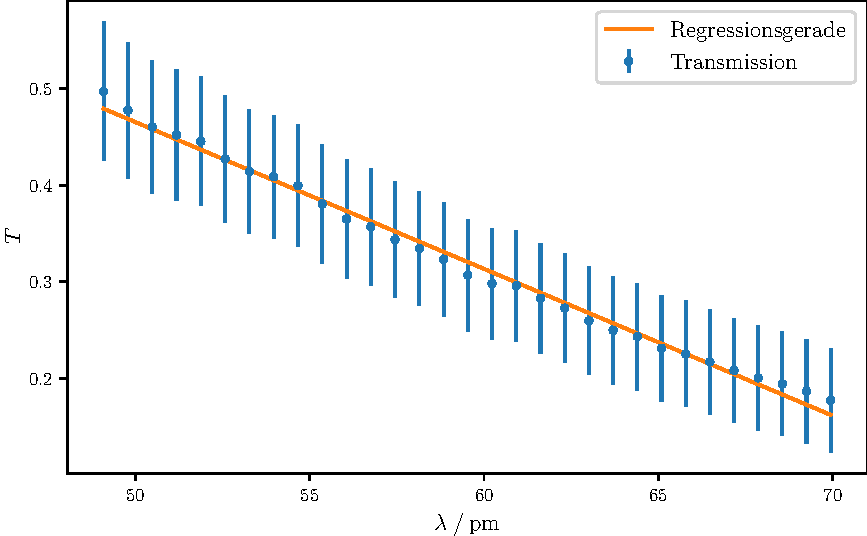
\includegraphics{build/transmission.pdf}
\end{figure}
Die in der Abbildung \ref{fig:Transmission} eingezeichnete Regressionsgerade hat die Form 
\begin{equation*}
    y = mx+b \; \text{,}
\end{equation*}
wobei sich die Parameter zu 
\begin{align*}
    m &= \num{1.519(24)e+10} \\
    b &= \num{1.225(14)}
\end{align*}
ergeben.
\FloatBarrier
\subsection{Bestimmung der Compton-Wellenlänge}
Zur Bestimmung der Compton-Wellenlänge wurden die Intensitäten 
\begin{align*}
    I_0 &= \num{2731(3)}\\
    I_1 &= \num{1180(2)}\\
    I_2 &= \num{1024(2)}
\end{align*}
gemessen. 
Hierbei ist keine Totzeitkorrektur\eqref{eqn:tot} nötig, da die gemessen Intensitäten und somit auch die Zählraten so gering sind,
so dass $\tau N << 1$ gilt.
Daraus ergeben sich Transmissionen von 
\begin{align*}
    T_1 &=\frac{I_1}{I_0} = 0.43 \\
    T_2 &=\frac{I_2}{I_0} = 0.37 \; \text{.}
\end{align*}
Um nun die dazugehörige Wellenlänge bestimmen zu können, wird die Regressionsgerade aus Abschnitt \ref{sec:transmission}
auf
\begin{equation*}
    x = \frac{y-b}{m}
\end{equation*}
umgestellt, wobei für y die eben berechneten Transmissionen $T$ und für $b$ bzw. $m$ die Werte für die Parameter der Regressionsgerade eingesetzt werden.
Daraus ergeben sich Wellenlänge. von 
\begin{align*}
    \lambda_1 &= \SI{52.19(125)}{\pico\metre} \\
    \lambda_2 &= \SI{55.95(129)}{\pico\metre} \; \text{.}
\end{align*}
Somit lässt sich die Compton-Wellenlänge zu 
\begin{equation*}
    \lambda_\text{c} = \SI{3.76(6)}{\pico\metre}
\end{equation*}
bestimmen lassen.